\documentclass[aspectratio=169,11pt]{beamer}
\usetheme{Madrid}
\usepackage[T1]{fontenc}
\usepackage{lmodern,graphicx,booktabs,tikz,array}
\newcolumntype{L}[1]{>{\raggedright\arraybackslash}p{#1}}
\definecolor{teamblue}{RGB}{25,55,90}
\setbeamercolor{structure}{fg=teamblue}
\setbeamercolor{frametitle}{bg=teamblue,fg=white}
\setbeamertemplate{navigation symbols}{}
\setbeamertemplate{footline}{\hfill\normalfont\tiny\insertframenumber\,/\,\inserttotalframenumber\hspace{2ex}\vspace{1ex}}
\title{Design Patterns in a Rails Booking Application}
\subtitle{Source evidence, requirement evolution and four-language comparison}
\author{Team A7\\\small Kavya Penikalapati \quad E. Abhijith Krishna\\\small Guduru Akshaya Giri \quad Kurt Sony Rebello}
\institute{23CSE455 -- B.Tech Artificial Intelligence \& Data Science}
\date{Submission date not verified from retained inputs}
\begin{document}
\begin{frame}\titlepage\end{frame}
\begin{frame}{A fixed baseline makes the findings reproducible}
\textbf{Application:} \texttt{andrewdsilva/rails-room-booking}
\begin{itemize}
\item Ruby 2.7.5, Rails 7.0.4 dependency and PostgreSQL configuration.
\item Commit: {\scriptsize\texttt{5e15551ee646871b4bed32c982fa17da319d3ee3}}.
\item Rails MVC and Active Record organize User, Room, Booking and Setting.
\item Devise, Pundit, Payify/Stripe and webhooks are integration boundaries.
\end{itemize}
\vspace{0.3cm}
\textbf{Method:} establish participant roles, calls and purpose in source before assigning a GoF pattern.
\end{frame}
\begin{frame}{One baseline collaboration supports Template Method}
\begin{columns}[T]
\begin{column}{0.48\textwidth}
\textbf{Stable CRUD skeleton}
\begin{enumerate}
\item Authorize and construct the resource.
\item Validate and save it.
\item Redirect on success, or render errors.
\end{enumerate}
\texttt{CrudConcern} is a Ruby module mixed into three controllers.
\end{column}
\begin{column}{0.48\textwidth}
\textbf{Resource hooks vary}
\begin{itemize}
\item \texttt{base\_class}, \texttt{object\_class}
\item \texttt{model\_params}, \texttt{strong\_params}
\item Settings overrides lookup and redirect.
\end{itemize}
Required hooks raise \texttt{NotImplementedError} in the shared module.
\end{column}
\end{columns}
\end{frame}
\begin{frame}{Module inclusion expresses the Rails collaboration}
\centering
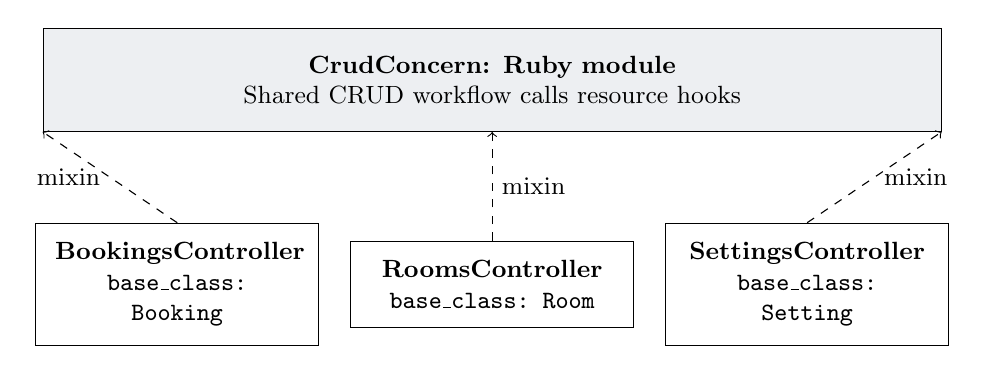
\begin{tikzpicture}[every node/.style={font=\small}]
\node[draw,fill=teamblue!8,text width=10.7cm,align=center,inner sep=10pt] (module) at (0,2.6) {\textbf{CrudConcern: Ruby module}\\Shared CRUD workflow calls resource hooks};
\node[draw,text width=3.1cm,align=center,inner sep=7pt] (booking) at (-4,0) {\textbf{BookingsController}\\\texttt{base\_class: Booking}};
\node[draw,text width=3.1cm,align=center,inner sep=7pt] (room) at (0,0) {\textbf{RoomsController}\\\texttt{base\_class: Room}};
\node[draw,text width=3.1cm,align=center,inner sep=7pt] (setting) at (4,0) {\textbf{SettingsController}\\\texttt{base\_class: Setting}};
\draw[dashed,->] (booking.north) -- (module.south west) node[midway,left] {mixin};
\draw[dashed,->] (room.north) -- (module.south) node[midway,right] {mixin};
\draw[dashed,->] (setting.north) -- (module.south east) node[midway,right] {mixin};
\end{tikzpicture}\par
\vspace{0.2cm}
\texttt{include ::CrudConcern} mixes in the skeleton.\\Controllers supply hooks and inherit ApplicationController.
\end{frame}
\begin{frame}{Framework vocabulary alone does not prove a pattern}
\begin{tabular}{L{0.24\linewidth}L{0.67\linewidth}}
\toprule Candidate & Evidence boundary\\\midrule
Observer & Callbacks do not establish application-owned observer objects.\\[0.15cm]
Strategy & Pundit policies do not establish the claimed interchangeable algorithm context.\\[0.15cm]
Decorator & A concern adds methods through module inclusion; runtime object wrapping is absent.\\[0.15cm]
Adapter / Facade & External Payify internals were not treated as application source.\\\bottomrule
\end{tabular}
\end{frame}
\begin{frame}{Four requirements create three distinct design pressures}
\begin{tabular}{L{0.27\linewidth}L{0.26\linewidth}L{0.37\linewidth}}
\toprule Requirement & Responsibility & Implementation\\\midrule
Breakfast / airport transfer & Optional booking services & AdditionalService subclasses and BookingService records\\[0.18cm]
Room upgrade & Reservation modification & RoomUpgrade checks availability and recalculates price\\[0.18cm]
Cancellation rules & Variable algorithms & CancellationService delegates to policy objects\\\bottomrule
\end{tabular}\par
\vspace{0.3cm}
Template Method remains; cancellation introduces Strategy. The other changes are domain modeling and responsibility extraction.
\end{frame}
\begin{frame}{Cancellation delegates refund rules to a Strategy}
\begin{columns}[T]
\begin{column}{0.48\textwidth}
\textbf{Context: CancellationService}
\begin{enumerate}
\item Ask the policy whether cancellation is permitted.
\item Ask it to calculate the refund.
\item Persist the cancellation time and calculated refund; return the result.
\end{enumerate}
\end{column}
\begin{column}{0.48\textwidth}
\textbf{Interchangeable policies}
\begin{itemize}
\item FlexibleCancellationPolicy
\item PartialRefundCancellationPolicy
\item NoRefundCancellationPolicy
\end{itemize}
A new rule changes the policy family without adding branches to the orchestration.
\end{column}
\end{columns}
\end{frame}
\begin{frame}{The two pattern ideas run in four languages}
\begin{tabular}{L{0.18\linewidth}L{0.70\linewidth}}
\toprule Language & Contract mechanism\\\midrule
Java & Abstract workflow class and policy interface\\[0.14cm]
Python & Abstract base classes and dynamic dispatch\\[0.14cm]
JavaScript & Class methods and runtime polymorphism\\[0.14cm]
C++ & Pure virtual methods and explicit ownership\\\bottomrule
\end{tabular}\par
\vspace{0.35cm}
Eight isolated snippets passed behavioral smoke checks. Strategy refunds for amount 430: full 430, partial 215, no refund 0.
\end{frame}
\begin{frame}{Process timing describes this environment}
\centering
\begin{tabular}{lrr}
\toprule Language & Template Method (ms) & Strategy (ms)\\\midrule
Java & 39.494 & 50.372\\
Python & 672.008 & 595.258\\
JavaScript & 21.401 & 21.762\\
C++ & 1.097 & 1.223\\\bottomrule
\end{tabular}\par
\vspace{0.4cm}\raggedright
One warmup, then five measured processes; median reported. Startup is included. Tiny examples and different runtimes prevent universal language-speed conclusions.
\end{frame}
\begin{frame}{Evidence determines the strength of each conclusion}
\begin{itemize}
\item Source traces establish Template Method and the introduced Strategy.
\item Part 3 outputs establish behavior of the eight isolated examples.
\item Fresh Rails verification: 36 examples, zero failures; all 12 migrations applied. Earlier HTTP startup receipt is retained separately.
\item Historical Prompt 02/03 wording and some model/date metadata were not retained; gaps are disclosed.
\end{itemize}
\vspace{0.3cm}
\textbf{Finding:} use a pattern when the collaboration and design pressure justify it. A smaller evidence-backed inventory is easier to defend.
\end{frame}
\begin{frame}{Cumulative source checkpoints make evolution reproducible}
\begin{itemize}
\item original: retained upstream source; Change3: final Rails application.
\item Change1/Change2 are reconstructed review stages, not historical commits.
\item Booking.active belongs to Change2, before RoomUpgrade calls it.
\item True unified patches replay each transition; hashes bind every source file.
\item Fresh cumulative RSpec suites: 5/0, 13/0, 21/0 and 36/0.
\end{itemize}
\end{frame}
\begin{frame}{Added functionality increases measured source complexity}
\centering
\begin{tabular}{lrrrr}
\toprule Stage & SLOC & Methods & Sum method CC & Explicit refs.\\\midrule
original & 495 & 95 & 127 & 27\\
Change1 & 556 & 105 & 145 & 31\\
Change2 & 596 & 110 & 154 & 31\\
Change3 & 654 & 121 & 171 & 35\\\bottomrule
\end{tabular}\par
\vspace{0.3cm}\raggedright
Ruby Ripper measurements of application Ruby files. Explicit constant references are a bounded coupling proxy, excluding implicit Rails dependencies. Cumulative stages add requirements; these are not quality scores or timing claims.
\end{frame}
\begin{frame}{Snapshot counts separate collaborations and participants}
\centering
\begin{tabular}{lrrrrr}
\toprule Snapshot & Types/instances & Concrete & Symbols & Rejected & Uncertain\\\midrule
original & 1/1 & 3 & 4 & 13 & 2\\
Change1 & 1/1 & 3 & 4 & 17 & 2\\
Change2 & 1/1 & 3 & 4 & 20 & 2\\
Change3 & 2/2 & 6 & 10 & 21 & 2\\\bottomrule
\end{tabular}\par
\vspace{0.3cm}\raggedright
Current source-review observations with reasons and source bounds. Shared symbols count once; the final policy selector is a callable, not an invented class. These are not recovered historical review events.
\end{frame}
\end{document}
